%==============================================================
%  EE201 -- Circuit Theory I
%  Lecture 2 : Kirchhoff's Laws   --   presentation slides
%  M. Mert Ankaralı, METU EEE
%
%  Compile:  ./build.sh      (or: pdflatex EE201_Lecture_2_slides.tex, twice)
%  Same colour code as the handout:
%      charge = purple, current = blue, voltage = orange, power = green
%==============================================================
\documentclass[11pt,aspectratio=169]{beamer}

\usepackage[T1]{fontenc}
\usepackage[utf8]{inputenc}
\usepackage[english]{babel}
\usepackage{lmodern}
\usepackage{amsmath,amssymb}
\usepackage{booktabs}
\usepackage{array}
\usepackage{colortbl}
\usepackage{tikz}
\usepackage[american,siunitx]{circuitikz}
\usetikzlibrary{arrows.meta,positioning,calc,decorations.pathreplacing,decorations.pathmorphing,decorations.markings}

%-------------------- plain METU-flavoured theme --------------
\usetheme{default}
\usecolortheme{default}
\useinnertheme{rectangles}
\setbeamertemplate{navigation symbols}{}
\setbeamertemplate{itemize items}[square]
\setbeamerfont{frametitle}{size=\large,series=\bfseries}
\setbeamerfont{title}{size=\LARGE,series=\bfseries}

\definecolor{metured}{RGB}{155,27,48}
\definecolor{metugray}{RGB}{88,89,91}
\definecolor{metulight}{RGB}{243,240,241}
\definecolor{ccur}{RGB}{0,102,170}
\definecolor{cvolt}{RGB}{214,120,0}
\definecolor{cpow}{RGB}{23,128,74}
\definecolor{ccharge}{RGB}{124,60,160}

\setbeamercolor{structure}{fg=metured}
\setbeamercolor{frametitle}{fg=metured,bg=}
\setbeamercolor{title}{fg=metured}
\setbeamercolor{normal text}{fg=black!88}
\setbeamercolor{block title}{fg=white,bg=metured}
\setbeamercolor{block body}{bg=metulight}
\setbeamercolor{alerted text}{fg=metured}

\setbeamertemplate{frametitle}{%
  \vspace{0.55em}%
  \usebeamerfont{frametitle}\usebeamercolor[fg]{frametitle}\insertframetitle\par
  \vspace{-0.2em}{\color{metured}\rule{\textwidth}{1pt}}\par\vspace{-0.2em}}

\setbeamertemplate{footline}{%
  \hbox{\begin{beamercolorbox}[wd=\paperwidth,ht=2.4ex,dp=1.4ex,leftskip=1.2em,rightskip=1.2em]{}%
  \tiny\color{metugray}\coursecode\ \textbar\ Lecture 2: Kirchhoff's Laws
  \hfill \insertframenumber/\inserttotalframenumber
  \end{beamercolorbox}}}

%-------------------- macros ----------------------------------
\newcommand{\coursecode}{EE201}
\newcommand{\term}{Fall 2026--2027}
\newcommand{\Icol}[1]{\textcolor{ccur}{#1}}
\newcommand{\Vcol}[1]{\textcolor{cvolt}{#1}}
\newcommand{\Pcol}[1]{\textcolor{cpow}{#1}}
\newcommand{\Qcol}[1]{\textcolor{ccharge}{#1}}
\newcommand{\uni}[1]{\,\mathrm{#1}}
\newcommand{\A}{\uni{A}} \newcommand{\V}{\uni{V}}
\newcommand{\W}{\uni{W}} \newcommand{\J}{\uni{J}}
\newcommand{\Cb}{\uni{C}} \newcommand{\s}{\uni{s}}

\ctikzset{bipoles/length=0.9cm, label/align=straight}
\tikzset{
  curarr/.style={-{Stealth[length=2.6mm]}, ccur, very thick},
  blk/.style={draw=metugray, fill=metulight, rounded corners=2pt,
              minimum height=1.25cm, text width=2.45cm, align=center, font=\scriptsize},
  flowarr/.style={-{Stealth[length=3mm]}, metured, very thick},
  thru/.style={-{Stealth[length=2.2mm]}, ccur, very thick},
  acr/.style={{Stealth[length=2mm]}-{Stealth[length=2mm]}, cvolt, very thick},
  pan/.style={draw=gray!35, fill=metulight, rounded corners=3pt,
              minimum width=3.0cm, minimum height=2.3cm},
  pcap/.style={font=\scriptsize\bfseries, text=metured},
  pol/.style={font=\small, text=cvolt},
  iar/.style={-{Stealth[length=2.4mm]}, ccur, very thick},
  gnode/.style={circle, fill=metured, inner sep=0pt, minimum size=4.2pt},
  glab/.style={font=\footnotesize, text=metured},
  surf/.style={draw=cpow, very thick, dashed, rounded corners=6pt},
  gbr/.style={metugray, thick, postaction={decorate, decoration={markings,
      mark=at position 0.58 with {\arrow{Stealth[length=2.4mm]}}}}},
}

\newcommand{\ohm}{\,\Omega}
\newcommand{\Req}{R_{\mathrm{eq}}}

\hypersetup{colorlinks=true,allcolors=metured}

\title{Lecture 2: Kirchhoff's Laws}
\subtitle{EE201 -- Circuit Theory I}
\author{M. Mert Ankaralı}
\institute{\small Department of Electrical and Electronics Engineering\\
           Middle East Technical University}
\date{}

%==============================================================
\begin{document}

%--------------------------------------------------------------
\begin{frame}[plain]
  \titlepage
  \vspace{-1.2em}
  \begin{center}\scriptsize\color{metugray}
    \Icol{$\blacksquare$}~current \quad \Vcol{$\blacksquare$}~voltage \quad
    \Pcol{$\blacksquare$}~power \quad {\color{metured}$\blacksquare$}~topology
  \end{center}
\end{frame}

%--------------------------------------------------------------
\begin{frame}{A circuit --- and what we do not yet know}
  \vfill
  \begin{center}
  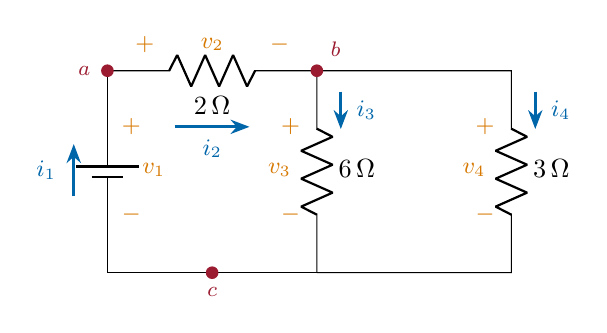
\begin{tikzpicture}[scale=0.95, transform shape]
      \draw (0,0) to[battery1, invert] (0,2.7);
      \draw (0,2.7) to[R, l_=$2\ohm$] (2.8,2.7);
      \draw (2.8,2.7) to[R, l=$6\ohm$] (2.8,0);
      \draw (2.8,2.7) -- (5.4,2.7) to[R, l=$3\ohm$] (5.4,0) -- (2.8,0);
      \draw (2.8,0) -- (0,0);
      \node[pol] at (0.32,1.95) {$+$}; \node[pol] at (0.32,0.78) {$-$};
      \node[pol] at (0.62,1.37) {$v_1$};
      \draw[iar] (-0.45,1.02) -- (-0.45,1.72); \node[ccur, font=\small] at (-0.82,1.37) {$i_1$};
      \node[pol] at (0.5,3.05) {$+$}; \node[pol] at (2.3,3.05) {$-$};
      \node[pol] at (1.4,3.05) {$v_2$};
      \draw[iar] (0.9,1.95) -- (1.9,1.95); \node[ccur, font=\small] at (1.4,1.66) {$i_2$};
      \node[pol] at (2.45,1.95) {$+$}; \node[pol] at (2.45,0.78) {$-$};
      \node[pol] at (2.3,1.37) {$v_3$};
      \draw[iar] (3.12,2.42) -- (3.12,1.92); \node[ccur, font=\small] at (3.46,2.17) {$i_3$};
      \node[pol] at (5.05,1.95) {$+$}; \node[pol] at (5.05,0.78) {$-$};
      \node[pol] at (4.9,1.37) {$v_4$};
      \draw[iar] (5.72,2.42) -- (5.72,1.92); \node[ccur, font=\small] at (6.06,2.17) {$i_4$};
      \fill[metured] (0,2.7) circle (2.4pt); \node[glab, left=3pt] at (0,2.7) {$a$};
      \fill[metured] (2.8,2.7) circle (2.4pt); \node[glab] at (3.05,2.99) {$b$};
      \fill[metured] (1.4,0) circle (2.4pt); \node[glab, below=2pt] at (1.4,0) {$c$};
  \end{tikzpicture}
  \end{center}
  \vfill
  \begin{center}
    Four branches, each carrying a \Vcol{voltage} and a \Icol{current}:\\[6pt]
    {\large $\Vcol{v_1},\Vcol{v_2},\Vcol{v_3},\Vcol{v_4}$ \quad and \quad
     $\Icol{i_1},\Icol{i_2},\Icol{i_3},\Icol{i_4}$ \qquad $\Longrightarrow$ \qquad
     \alert{$2b = 8$ unknowns}}
  \end{center}
  \vfill
\end{frame}

%--------------------------------------------------------------
\begin{frame}{Node, branch, loop}
  \vfill
  \begin{center}
  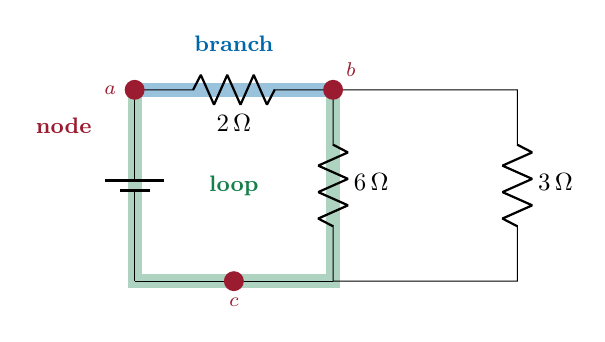
\begin{tikzpicture}[scale=0.9, transform shape]
    \draw[cpow!35, line width=5pt] (0,2.7) -- (0,0) -- (2.8,0) -- (2.8,2.7) -- (0,2.7);
    \draw[ccur!40, line width=5pt] (0,2.7) -- (2.8,2.7);
    \draw (0,0) to[battery1, invert] (0,2.7);
    \draw (0,2.7) to[R, l_=$2\ohm$] (2.8,2.7);
    \draw (2.8,2.7) to[R, l=$6\ohm$] (2.8,0);
    \draw (2.8,2.7) -- (5.4,2.7) to[R, l=$3\ohm$] (5.4,0) -- (2.8,0);
    \draw (2.8,0) -- (0,0);
    \fill[metured] (0,2.7) circle (4pt); \node[glab, left=4pt] at (0,2.7) {$a$};
    \fill[metured] (2.8,2.7) circle (4pt); \node[glab] at (3.05,2.99) {$b$};
    \fill[metured] (1.4,0) circle (4pt); \node[glab, below=3pt] at (1.4,0) {$c$};
    \node[font=\small\bfseries, text=ccur] at (1.4,3.35) {branch};
    \node[font=\small\bfseries, text=cpow] at (1.4,1.35) {loop};
    \node[font=\small\bfseries, text=metured] at (-1.0,2.2) {node};
  \end{tikzpicture}
  \end{center}
  \vfill
  \begin{center}\small
  \begin{minipage}{0.90\textwidth}
    \textbf{Node} --- a connection point; everything joined by ideal wire is \emph{one}
    node, no matter how much wire is drawn. Here $n = 3$.\\[3pt]
    \textbf{Branch} --- one element, two nodes. Here $b = 4$.\\[3pt]
    \textbf{Loop} --- a closed path through no node twice.
  \end{minipage}
  \end{center}
  \vfill
\end{frame}

%--------------------------------------------------------------
\begin{frame}{What each element says --- on its own}
  \vfill
  \begin{center}
  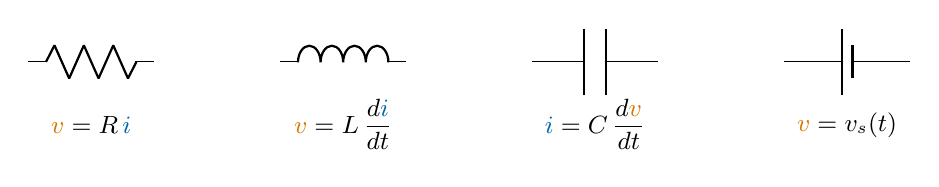
\begin{tikzpicture}[scale=1.0]
    \begin{scope}
      \draw (0,0) to[R] (1.6,0);
      \node[font=\small] at (0.8,-0.8) {$\Vcol{v} = R\,\Icol{i}$};
    \end{scope}
    \begin{scope}[xshift=3.2cm]
      \draw (0,0) to[L] (1.6,0);
      \node[font=\small] at (0.8,-0.8) {$\Vcol{v} = L\,\dfrac{d\Icol{i}}{dt}$};
    \end{scope}
    \begin{scope}[xshift=6.4cm]
      \draw (0,0) to[C] (1.6,0);
      \node[font=\small] at (0.8,-0.8) {$\Icol{i} = C\,\dfrac{d\Vcol{v}}{dt}$};
    \end{scope}
    \begin{scope}[xshift=9.6cm]
      \draw (0,0) to[battery1] (1.6,0);
      \node[font=\small] at (0.8,-0.8) {$\Vcol{v} = v_s(t)$};
    \end{scope}
  \end{tikzpicture}
  \end{center}
  \vfill
  \begin{center}
    For our circuit: \quad
    $\Vcol{v_1} = 12\V$, \ \ $\Vcol{v_2} = 2\,\Icol{i_2}$, \ \
    $\Vcol{v_3} = 6\,\Icol{i_3}$, \ \ $\Vcol{v_4} = 3\,\Icol{i_4}$
  \end{center}
  \vfill
  \begin{center}
    That is \alert{4 equations for 8 unknowns}. Exactly half ---\\
    and staring harder at the elements will never produce the rest.
  \end{center}
  \vfill
\end{frame}

%--------------------------------------------------------------
\begin{frame}{Two kinds of equations --- and they never mix}
  \vfill
  \begin{center}
  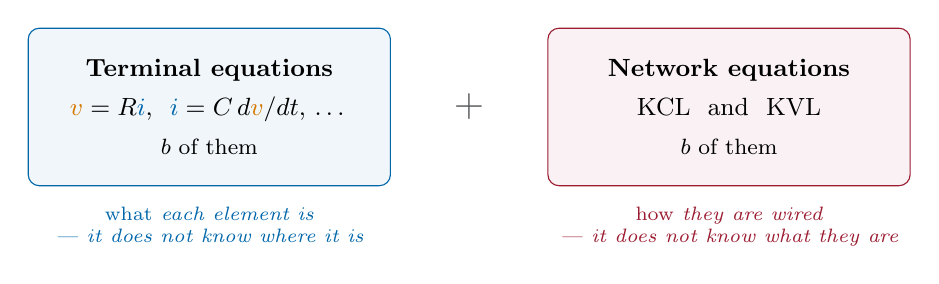
\begin{tikzpicture}[scale=1.0]
    \node[draw=ccur, fill=ccur!6, rounded corners=4pt, minimum width=4.6cm,
          minimum height=2.0cm, align=center, font=\small] (t) at (0,0)
         {\textbf{Terminal equations}\\[3pt] $\Vcol{v}=R\Icol{i}$, \ $\Icol{i}=C\,d\Vcol{v}/dt$, \dots\\[3pt]
          \footnotesize $b$ of them};
    \node[draw=metured, fill=metured!6, rounded corners=4pt, minimum width=4.6cm,
          minimum height=2.0cm, align=center, font=\small] (n) at (6.6,0)
         {\textbf{Network equations}\\[3pt] KCL \ and \ KVL\\[3pt]
          \footnotesize $b$ of them};
    \node[font=\Large, text=metugray] at (3.3,0) {$+$};
    \node[font=\scriptsize\itshape, text=ccur, align=center, below=4pt of t]
         {\emph{what} each element is\\ --- it does not know where it is};
    \node[font=\scriptsize\itshape, text=metured, align=center, below=4pt of n]
         {\emph{how} they are wired\\ --- it does not know what they are};
  \end{tikzpicture}
  \end{center}
  \vfill
  \begin{center}
    Because KCL and KVL ignore the elements, they hold for \alert{every} lumped
    circuit ---\\ linear or not, time-invariant or not, at DC or at $100\uni{MHz}$.
  \end{center}
  \vfill
\end{frame}

%--------------------------------------------------------------
\begin{frame}{Kirchhoff's Current Law}
  \vfill
  \begin{center}
    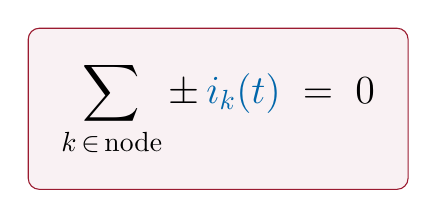
\begin{tikzpicture}
      \node[draw=metured, fill=metured!6, rounded corners=4pt, inner sep=12pt]
      {\Large $\displaystyle \sum_{k \,\in\, \text{node}} \pm\, \Icol{i_k(t)} \;=\; 0$};
    \end{tikzpicture}
  \end{center}
  \vfill
  \begin{center}
    at \alert{every node}, at \alert{every instant}.\\[6pt]
    {\large \emph{What flows in, flows out.}}
  \end{center}
  \vfill
\end{frame}

%--------------------------------------------------------------
\begin{frame}{Why: a node cannot store charge}
  \vfill
  \begin{center}
  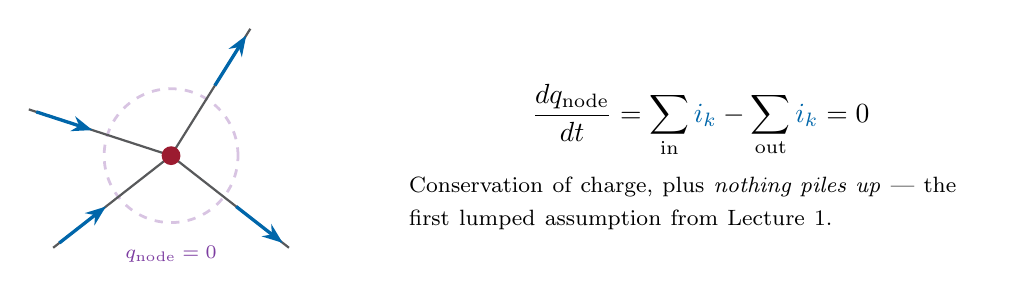
\begin{tikzpicture}[scale=1.0]
    \draw[ccharge!30, line width=1pt, dashed] (0,0) circle (0.85);
    \foreach \a in {162,58,-38,-142}{\draw[metugray, thick] (0,0) -- (\a:1.9);}
    \fill[metured] (0,0) circle (3.4pt);
    \draw[curarr] (162:1.80) -- (162:1.05);
    \draw[curarr] (58:1.05) -- (58:1.80);
    \draw[curarr] (-38:1.05) -- (-38:1.80);
    \draw[curarr] (-142:1.80) -- (-142:1.05);
    \node[font=\scriptsize, text=ccharge] at (0,-1.25) {$q_{\text{node}} = 0$};
    \node[font=\normalsize, anchor=west, text width=7.4cm] at (2.9,0)
      {\[ \frac{dq_{\text{node}}}{dt}
          = \sum_{\text{in}} \Icol{i_k} - \sum_{\text{out}} \Icol{i_k} = 0 \]
       \footnotesize Conservation of charge, plus \emph{nothing piles up} ---
       the first lumped assumption from Lecture 1.};
  \end{tikzpicture}
  \end{center}
  \vfill
\end{frame}

%--------------------------------------------------------------
\begin{frame}{Sign rule, and an example}
  \vfill
  \begin{columns}[c,onlytextwidth]
    \begin{column}{0.44\textwidth}
      \begin{center}
      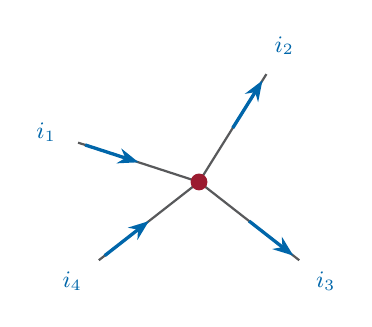
\begin{tikzpicture}[scale=0.95, transform shape]
        \foreach \a in {162,58,-38,-142}{\draw[metugray, thick] (0,0) -- (\a:1.7);}
        \fill[metured] (0,0) circle (3.2pt);
        \draw[curarr] (162:1.60) -- (162:0.85);
        \draw[curarr] (58:0.85) -- (58:1.60);
        \draw[curarr] (-38:0.85) -- (-38:1.60);
        \draw[curarr] (-142:1.60) -- (-142:0.85);
        \node[ccur, font=\small] at (162:2.15) {$i_1$};
        \node[ccur, font=\small] at (58:2.15) {$i_2$};
        \node[ccur, font=\small] at (-38:2.15) {$i_3$};
        \node[ccur, font=\small] at (-142:2.15) {$i_4$};
      \end{tikzpicture}
      \end{center}
    \end{column}
    \begin{column}{0.54\textwidth}
      \textbf{Leaving positive:}
      \[ -\Icol{i_1} + \Icol{i_2} + \Icol{i_3} - \Icol{i_4} = 0 \]
      \vspace{2pt}
      Given $\Icol{i_1} = 3\A$, \ $\Icol{i_2} = -2\A$, \ $\Icol{i_3} = 6\A$, \
      what is $\Icol{i_4}$?
      \onslide<2->
      \[ -3 + (-2) + 6 - \Icol{i_4} = 0 \;\Longrightarrow\; \alert{\Icol{i_4} = 1\A} \]
      \vspace{2pt}
      {\small A measured $-2\A$ goes in \emph{with its sign}. We never redraw the arrow.}
    \end{column}
  \end{columns}
  \vfill
\end{frame}

%--------------------------------------------------------------
\begin{frame}{Nothing in the argument needed a \alert{point}}
  \vfill
  \begin{center}
  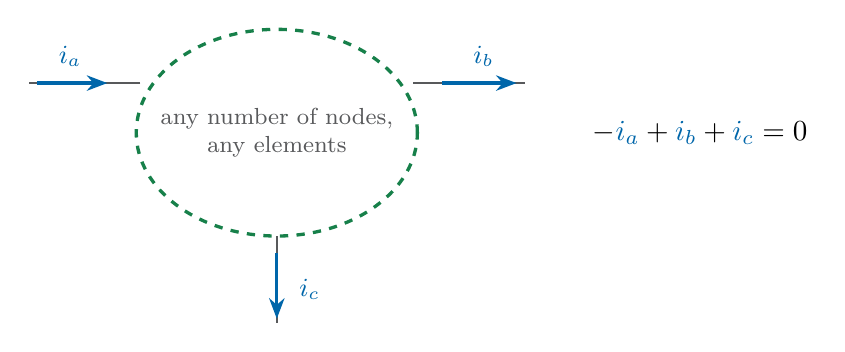
\begin{tikzpicture}[scale=1.05, transform shape]
    \draw[surf] (0,0) ellipse (1.7cm and 1.25cm);
    \node[font=\footnotesize, text=metugray, align=center] at (0,0)
         {any number of nodes,\\ any elements};
    \draw[metugray, thick] (-1.65,0.6) -- (-3.0,0.6);
    \draw[metugray, thick] (1.65,0.6) -- (3.0,0.6);
    \draw[metugray, thick] (0,-1.25) -- (0,-2.3);
    \draw[curarr] (-2.9,0.6) -- (-2.05,0.6);
    \draw[curarr] (2.0,0.6) -- (2.9,0.6);
    \draw[curarr] (0,-1.45) -- (0,-2.25);
    \node[ccur, font=\small, above] at (-2.5,0.68) {$i_a$};
    \node[ccur, font=\small, above] at (2.5,0.68) {$i_b$};
    \node[ccur, font=\small, right] at (0.15,-1.9) {$i_c$};
    \node[font=\normalsize, anchor=west] at (3.7,0)
      {$-\Icol{i_a} + \Icol{i_b} + \Icol{i_c} = 0$};
  \end{tikzpicture}
  \end{center}
  \vfill
  \begin{center}
    Only the branches that \alert{cross} the surface appear. One node or a thousand,
    resistors or a whole amplifier --- it makes no difference.
  \end{center}
  \vfill
\end{frame}

%--------------------------------------------------------------
\begin{frame}{Consequence I: series means \alert{one} current}
  \vfill
  \begin{center}
  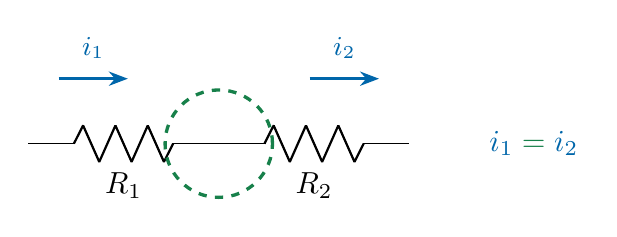
\begin{tikzpicture}[scale=1.1, transform shape]
    \draw (0,0) to[R, l_=$R_1$] (2.2,0) to[R, l_=$R_2$] (4.4,0);
    \draw[surf] (2.2,0) circle (0.62cm);
    \draw[iar] (0.35,0.75) -- (1.15,0.75);
    \draw[iar] (3.25,0.75) -- (4.05,0.75);
    \node[ccur, font=\small] at (0.75,1.1) {$i_1$};
    \node[ccur, font=\small] at (3.65,1.1) {$i_2$};
    \node[font=\normalsize, text=cpow, anchor=west] at (5.2,0) {$\Icol{i_1} = \Icol{i_2}$};
  \end{tikzpicture}
  \end{center}
  \vfill
  \begin{center}
    Exactly two branches cross the surface. A chain of elements has \alert{one} current
    ---\\ and that \emph{is} the definition of ``in series''.
  \end{center}
  \vfill
\end{frame}

%--------------------------------------------------------------
\begin{frame}{Consequence II: a box gives back what it takes}
  \vfill
  \begin{center}
  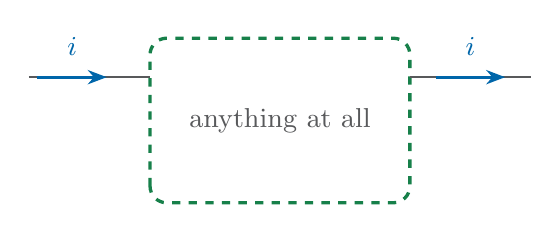
\begin{tikzpicture}[scale=1.1, transform shape]
    \draw[surf] (0,0) rectangle (3.0,1.9);
    \node[font=\small, text=metugray] at (1.5,0.95) {anything at all};
    \draw[metugray, thick] (-1.4,1.45) -- (0,1.45);
    \draw[metugray, thick] (3.0,1.45) -- (4.4,1.45);
    \draw[iar] (-1.3,1.45) -- (-0.5,1.45);
    \draw[iar] (3.3,1.45) -- (4.1,1.45);
    \node[ccur, font=\small] at (-0.9,1.8) {$i$};
    \node[ccur, font=\small] at (3.7,1.8) {$i$};
  \end{tikzpicture}
  \end{center}
  \vfill
  \begin{center}
    This is what lets us say ``\alert{the} current through'' a black box ---\\
    and what makes a two-terminal element a meaningful idea at all.
  \end{center}
  \vfill
\end{frame}

%--------------------------------------------------------------
\begin{frame}{Two things KCL is not}
  \vfill
  \begin{center}
  \begin{columns}[T,onlytextwidth]
    \begin{column}{0.46\textwidth}
      \begin{block}{Not averaged}
        \small $\sum \pm \Icol{i_k(t)} = 0$ holds at each instant $t$ \emph{separately}.
        Nothing is averaged over time.
      \end{block}
    \end{column}
    \begin{column}{0.46\textwidth}
      \begin{block}{Not about $v$}
        \small It says nothing about voltage, resistance or power. Topology and current
        only.
      \end{block}
    \end{column}
  \end{columns}
  \end{center}
  \vfill
\end{frame}

%--------------------------------------------------------------
\begin{frame}{Kirchhoff's Voltage Law}
  \vfill
  \begin{center}
    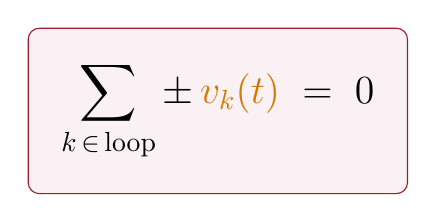
\begin{tikzpicture}
      \node[draw=metured, fill=metured!6, rounded corners=4pt, inner sep=12pt]
      {\Large $\displaystyle \sum_{k \,\in\, \text{loop}} \pm\, \Vcol{v_k(t)} \;=\; 0$};
    \end{tikzpicture}
  \end{center}
  \vfill
  \begin{center}
    round \alert{every loop}, at \alert{every instant}.\\[6pt]
    {\large \emph{Go all the way round and you come back to where you started.}}
  \end{center}
  \vfill
  \begin{center}\small\color{metugray}
    As with KCL, this is the lumped model at work: it holds as long as no magnetic field
    is changing through the loop --- assumption (b) from Lecture 1.
  \end{center}
  \vfill
\end{frame}

%--------------------------------------------------------------
\begin{frame}{Why: the differences telescope}
  \vfill
  \begin{center}
  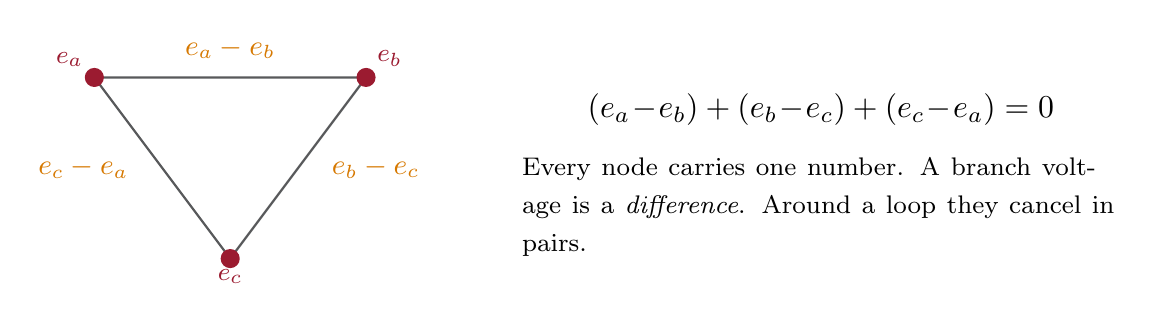
\begin{tikzpicture}[scale=1.15, transform shape]
    \coordinate (A) at (0,0); \coordinate (B) at (3.0,0); \coordinate (C) at (1.5,-2.0);
    \draw[metugray, thick] (A) -- (B) -- (C) -- (A);
    \fill[metured] (A) circle (3pt); \fill[metured] (B) circle (3pt);
    \fill[metured] (C) circle (3pt);
    \node[glab, above left] at (A) {$e_a$}; \node[glab, above right] at (B) {$e_b$};
    \node[glab, below] at (C) {$e_c$};
    \node[cvolt, font=\small] at (1.5,0.32) {$e_a - e_b$};
    \node[cvolt, font=\small, anchor=west] at (2.5,-1.0) {$e_b - e_c$};
    \node[cvolt, font=\small, anchor=east] at (0.5,-1.0) {$e_c - e_a$};
    \node[font=\normalsize, anchor=west, text width=6.6cm] at (4.6,-1.0)
      {\[ (e_a\!-\!e_b) + (e_b\!-\!e_c) + (e_c\!-\!e_a) = 0 \]
       \footnotesize Every node carries one number. A branch voltage is a
       \emph{difference}. Around a loop they cancel in pairs.};
  \end{tikzpicture}
  \end{center}
  \vfill
\end{frame}

%--------------------------------------------------------------
\begin{frame}{Sign rule: walk the loop}
  \vfill
  \begin{columns}[c,onlytextwidth]
    \begin{column}{0.52\textwidth}
      \begin{center}
      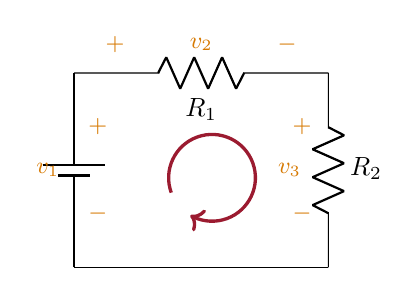
\begin{tikzpicture}[scale=0.95, transform shape]
        \draw (0,0) to[battery1, invert] (0,2.6);
        \draw (0,2.6) to[R, l_=$R_1$] (3.4,2.6);
        \draw (3.4,2.6) to[R, l=$R_2$] (3.4,0);
        \draw (3.4,0) -- (0,0);
        \node[pol] at (0.32,1.88) {$+$}; \node[pol] at (0.32,0.72) {$-$};
        \node[pol] at (-0.35,1.30) {$v_1$};
        \node[pol] at (0.55,2.98) {$+$}; \node[pol] at (2.85,2.98) {$-$};
        \node[pol] at (1.7,2.98) {$v_2$};
        \node[pol] at (3.05,1.88) {$+$}; \node[pol] at (3.05,0.72) {$-$};
        \node[pol] at (2.88,1.30) {$v_3$};
        \draw[metured, very thick, ->] (1.30,1.00) arc (200:-120:0.58);
      \end{tikzpicture}
      \end{center}
    \end{column}
    \begin{column}{0.46\textwidth}
      \[ -\Vcol{v_1} + \Vcol{v_2} + \Vcol{v_3} = 0 \]
      \vspace{4pt}
      \begin{itemize}\itemsep5pt
        \item $+$ when you traverse a branch from $+$ to $-$;
        \item $-$ when you go the other way.
      \end{itemize}
      \vspace{4pt}
      {\small Walking anticlockwise multiplies every term by $-1$ --- same equation.}
    \end{column}
  \end{columns}
  \vfill
\end{frame}

%--------------------------------------------------------------
\begin{frame}{The same statement: voltage forgets the path}
  \vfill
  \begin{center}
  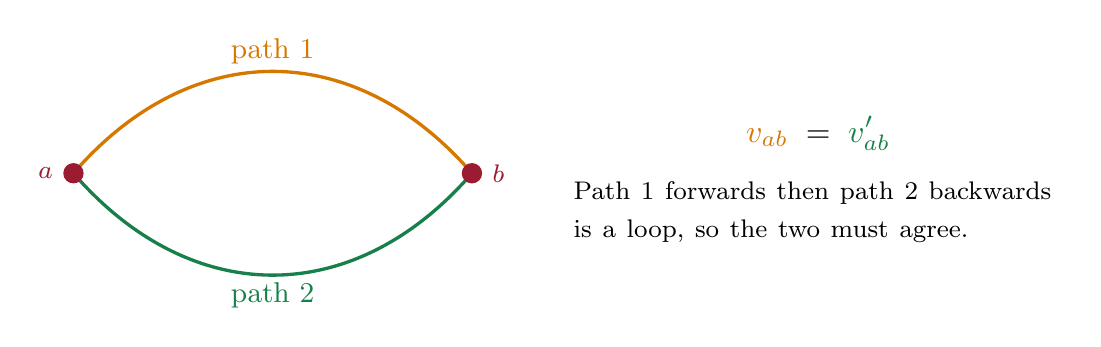
\begin{tikzpicture}[scale=1.15, transform shape]
    \coordinate (A) at (0,0); \coordinate (B) at (4.4,0);
    \draw[cvolt, very thick] (A) .. controls (1.3,1.5) and (3.1,1.5) .. (B);
    \draw[cpow, very thick] (A) .. controls (1.3,-1.5) and (3.1,-1.5) .. (B);
    \fill[metured] (A) circle (3.2pt); \fill[metured] (B) circle (3.2pt);
    \node[glab, left=3pt] at (A) {$a$}; \node[glab, right=3pt] at (B) {$b$};
    \node[cvolt, font=\small] at (2.2,1.35) {path 1};
    \node[cpow, font=\small] at (2.2,-1.35) {path 2};
    \node[font=\normalsize, anchor=west, text width=5.4cm] at (5.4,0)
      {\[ \Vcol{v_{ab}} \;=\; \Pcol{v'_{ab}} \]
       \footnotesize Path 1 forwards then path 2 backwards is a loop,
       so the two must agree.};
  \end{tikzpicture}
  \end{center}
  \vfill
  \begin{center}
    This is why ``the voltage across $R_2$'' means something ---\\
    and why node potentials exist at all.
  \end{center}
  \vfill
\end{frame}

%--------------------------------------------------------------
\begin{frame}{Example: one loop}
  \vfill
  \begin{columns}[c,onlytextwidth]
    \begin{column}{0.45\textwidth}
      \begin{center}
      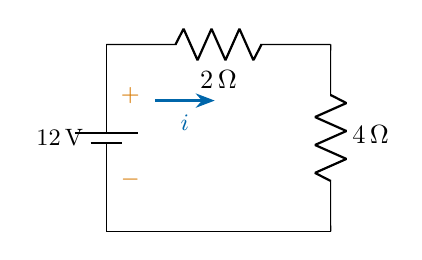
\begin{tikzpicture}[scale=0.95, transform shape]
        \draw (0,0) to[battery1, invert] (0,2.5);
        \draw (0,2.5) to[R, l_=$2\ohm$] (3.0,2.5);
        \draw (3.0,2.5) to[R, l=$4\ohm$] (3.0,0);
        \draw (3.0,0) -- (0,0);
        \node[pol] at (0.32,1.82) {$+$}; \node[pol] at (0.32,0.70) {$-$};
        \node[font=\small] at (-0.62,1.26) {$12\V$};
        \draw[iar] (0.65,1.75) -- (1.45,1.75); \node[ccur, font=\small] at (1.05,1.46) {$i$};
      \end{tikzpicture}
      \end{center}
    \end{column}
    \begin{column}{0.53\textwidth}
      \begin{center}\small Walk the loop. What is $\Icol{i}$?\end{center}
      \onslide<2->
      \[ -12 + 2\Icol{i} + 4\Icol{i} = 0 \]
      \[ \Longrightarrow\quad \alert{\Icol{i} = 2\A} \]
      \vspace{2pt}
      \onslide<3->
      \[ \Vcol{v_{2\Omega}} = 4\V, \qquad \Vcol{v_{4\Omega}} = 8\V \]
      \vspace{2pt}
      \begin{center}\small
        $4 + 8 = 12$: the source's volts are shared in proportion to resistance.
      \end{center}
    \end{column}
  \end{columns}
  \vfill
\end{frame}

%--------------------------------------------------------------
\begin{frame}{Example: three loops, two equations}
  \vfill
  \begin{center}
  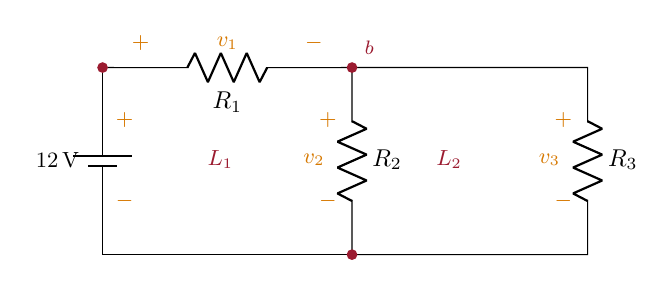
\begin{tikzpicture}[scale=0.88, transform shape]
    \draw (0,0) to[battery1, invert] (0,2.7);
    \draw (0,2.7) to[R, l_=$R_1$] (3.6,2.7);
    \draw (3.6,2.7) to[R, l=$R_2$] (3.6,0);
    \draw (3.6,2.7) -- (7.0,2.7) to[R, l=$R_3$] (7.0,0) -- (3.6,0);
    \draw (3.6,0) -- (0,0);
    \node[pol] at (0.32,1.95) {$+$}; \node[pol] at (0.32,0.78) {$-$};
    \node[font=\small] at (-0.65,1.37) {$12\V$};
    \node[pol] at (0.55,3.05) {$+$}; \node[pol] at (3.05,3.05) {$-$};
    \node[pol] at (1.8,3.05) {$v_1$};
    \node[pol] at (3.25,1.95) {$+$}; \node[pol] at (3.25,0.78) {$-$};
    \node[pol] at (3.05,1.37) {$v_2$};
    \node[pol] at (6.65,1.95) {$+$}; \node[pol] at (6.65,0.78) {$-$};
    \node[pol] at (6.45,1.37) {$v_3$};
    \node[metured, font=\small\itshape] at (1.7,1.37) {$L_1$};
    \node[metured, font=\small\itshape] at (5.0,1.37) {$L_2$};
    \fill[metured] (0,2.7) circle (2.2pt);
    \fill[metured] (3.6,2.7) circle (2.2pt); \node[glab] at (3.85,2.99) {$b$};
    \fill[metured] (3.6,0) circle (2.2pt);
  \end{tikzpicture}
  \end{center}
  \vfill
  \begin{center}
  $L_1: \; -12 + \Vcol{v_1} + \Vcol{v_2} = 0$ \qquad
  $L_2: \; -\Vcol{v_2} + \Vcol{v_3} = 0$ \qquad
  \onslide<2->{$\underbrace{L_3: \; -12 + \Vcol{v_1} + \Vcol{v_3} = 0}_{\textstyle =\, L_1 + L_2}$}
  \end{center}
  \vfill
  \begin{center}
    \onslide<2->{The third loop is \alert{true but not new}. Only $\ell = b - n + 1 = 2$
    of them count.}
  \end{center}
  \vfill
\end{frame}

%--------------------------------------------------------------
\begin{frame}{The whole bookkeeping, on one slide}
  \vfill
  \begin{center}\small
    $n$ = number of \alert{nodes}, \quad $b$ = number of \alert{branches}. \quad
    Here $n = 3$, $b = 4$.
  \end{center}
  \vfill
  \begin{center}
  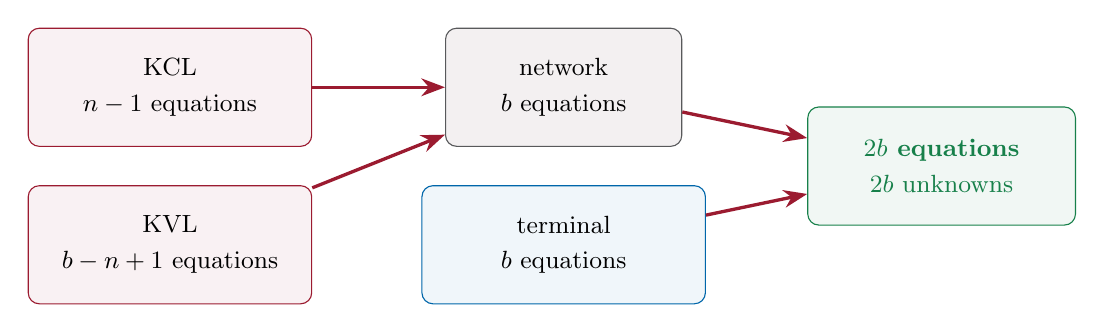
\begin{tikzpicture}[scale=1.0]
    \node[draw=metured, fill=metured!6, rounded corners=4pt, minimum width=3.6cm,
          minimum height=1.5cm, align=center, font=\small] (k) at (0,1.1)
         {KCL\\[2pt] $n-1$ equations};
    \node[draw=metured, fill=metured!6, rounded corners=4pt, minimum width=3.6cm,
          minimum height=1.5cm, align=center, font=\small] (v) at (0,-0.9)
         {KVL\\[2pt] $b-n+1$ equations};
    \node[draw=ccur, fill=ccur!6, rounded corners=4pt, minimum width=3.6cm,
          minimum height=1.5cm, align=center, font=\small] (t) at (5.0,-0.9)
         {terminal\\[2pt] $b$ equations};
    \node[draw=metugray, fill=metulight, rounded corners=4pt, minimum width=3.0cm,
          minimum height=1.5cm, align=center, font=\small] (s) at (5.0,1.1)
         {network\\[2pt] $b$ equations};
    \draw[flowarr] (k) -- (s); \draw[flowarr] (v) -- (s);
    \node[draw=cpow, fill=cpow!6, rounded corners=4pt, minimum width=3.4cm,
          minimum height=1.5cm, align=center, font=\small, text=cpow] (tot) at (9.8,0.1)
         {\textbf{$2b$ equations}\\[2pt] $2b$ unknowns};
    \draw[flowarr] (s) -- (tot); \draw[flowarr] (t) -- (tot);
  \end{tikzpicture}
  \end{center}
  \vfill
  \begin{center}\small
    \textbf{Why is one KCL redundant?} Each branch current leaves one node and enters
    another, so it appears in exactly two node equations --- once with $+$, once with
    $-$. Add all $n$ of them and every current cancels: $0 = 0$. Whichever node you drop,
    its equation can be rebuilt from the rest, so only $n-1$ say anything new.
  \end{center}
  \vfill
\end{frame}

%--------------------------------------------------------------
\begin{frame}{Some diagrams mean nothing at all}
  \vfill
  \begin{center}
  \begin{tikzpicture}[scale=0.88, transform shape]
    % two voltage sources in parallel
    \begin{scope}
      \draw (0,0) to[battery1, invert] (0,2.2);
      \draw (2.4,0) to[battery1, invert] (2.4,2.2);
      \draw (0,2.2) -- (2.4,2.2); \draw (0,0) -- (2.4,0);
      \node[font=\small] at (-0.65,1.1) {$5\V$};
      \node[font=\small] at (3.05,1.1) {$9\V$};
      \fill[metured] (1.2,2.2) circle (2.4pt); \fill[metured] (1.2,0) circle (2.4pt);
      \node[font=\small, text=metured] at (1.2,-0.85) {KVL: \ $5 = 9$};
    \end{scope}
    % two current sources in series
    \begin{scope}[xshift=6.6cm, yshift=0.5cm]
      \draw (0,0) to[american current source] (2.0,0);
      \draw (2.0,0) to[american current source] (4.0,0);
      \draw (4.0,0) -- (4.0,-1.4) -- (0,-1.4) -- (0,0);
      \node[font=\small] at (1.0,0.75) {$2\A$};
      \node[font=\small] at (3.0,0.75) {$3\A$};
      \fill[metured] (2.0,0) circle (2.4pt);
      \node[font=\small, text=metured] at (2.0,-2.05) {KCL: \ $2 = 3$};
    \end{scope}
  \end{tikzpicture}
  \end{center}
  \vfill
  \begin{center}
    Both are \alert{false whatever the other variables do} --- the diagram describes no
    circuit. An ideal source promises to hold its value at any cost, and two such promises
    can disagree.\\[5pt]
    {\small\color{metugray} Give each source its internal resistance and the equations
    agree again, with a very large current. Sometimes that is harmless; sometimes it is
    why one of them makes smoke.}
  \end{center}
  \vfill
\end{frame}

%--------------------------------------------------------------
\begin{frame}{All $2b$ equations, once}
  \vfill
  \begin{columns}[c,onlytextwidth]
    \begin{column}{0.47\textwidth}
      \begin{center}
      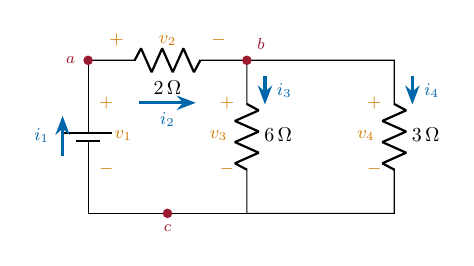
\begin{tikzpicture}[scale=0.72, transform shape]
        \draw (0,0) to[battery1, invert] (0,2.7);
        \draw (0,2.7) to[R, l_=$2\ohm$] (2.8,2.7);
        \draw (2.8,2.7) to[R, l=$6\ohm$] (2.8,0);
        \draw (2.8,2.7) -- (5.4,2.7) to[R, l=$3\ohm$] (5.4,0) -- (2.8,0);
        \draw (2.8,0) -- (0,0);
        \node[pol] at (0.32,1.95) {$+$}; \node[pol] at (0.32,0.78) {$-$};
        \node[pol] at (0.62,1.37) {$v_1$};
        \draw[iar] (-0.45,1.02) -- (-0.45,1.72); \node[ccur, font=\small] at (-0.82,1.37) {$i_1$};
        \node[pol] at (0.5,3.05) {$+$}; \node[pol] at (2.3,3.05) {$-$};
        \node[pol] at (1.4,3.05) {$v_2$};
        \draw[iar] (0.9,1.95) -- (1.9,1.95); \node[ccur, font=\small] at (1.4,1.66) {$i_2$};
        \node[pol] at (2.45,1.95) {$+$}; \node[pol] at (2.45,0.78) {$-$};
        \node[pol] at (2.3,1.37) {$v_3$};
        \draw[iar] (3.12,2.42) -- (3.12,1.92); \node[ccur, font=\small] at (3.46,2.17) {$i_3$};
        \node[pol] at (5.05,1.95) {$+$}; \node[pol] at (5.05,0.78) {$-$};
        \node[pol] at (4.9,1.37) {$v_4$};
        \draw[iar] (5.72,2.42) -- (5.72,1.92); \node[ccur, font=\small] at (6.06,2.17) {$i_4$};
        \fill[metured] (0,2.7) circle (2.4pt); \node[glab, left=3pt] at (0,2.7) {$a$};
        \fill[metured] (2.8,2.7) circle (2.4pt); \node[glab] at (3.05,2.99) {$b$};
        \fill[metured] (1.4,0) circle (2.4pt); \node[glab, below=2pt] at (1.4,0) {$c$};
      \end{tikzpicture}
      \end{center}
    \end{column}
    \begin{column}{0.51\textwidth}
      \footnotesize
      \begin{tabular}{@{}l@{\hspace{1.0em}}l@{}}
        \multicolumn{2}{@{}l}{\textbf{terminal (4)}}\\
        $\Vcol{v_1} = 12$ & $\Vcol{v_3} = 6\,\Icol{i_3}$\\
        $\Vcol{v_2} = 2\,\Icol{i_2}$ & $\Vcol{v_4} = 3\,\Icol{i_4}$\\[6pt]
        \multicolumn{2}{@{}l}{\onslide<2->{\textbf{KCL (2)}}}\\
        \multicolumn{2}{@{}l}{\onslide<2->{$a$: \ $-\Icol{i_1}+\Icol{i_2}=0$ \qquad
                               $b$: \ $-\Icol{i_2}+\Icol{i_3}+\Icol{i_4}=0$}}\\[6pt]
        \multicolumn{2}{@{}l}{\onslide<3->{\textbf{KVL (2)}}}\\
        \multicolumn{2}{@{}l}{\onslide<3->{$L_1$: \ $-\Vcol{v_1}+\Vcol{v_2}+\Vcol{v_3}=0$}}\\
        \multicolumn{2}{@{}l}{\onslide<3->{$L_2$: \ $-\Vcol{v_3}+\Vcol{v_4}=0$}}\\
      \end{tabular}
      \vspace{6pt}
      \begin{center}
      \onslide<4->{$\Icol{i_1}=\Icol{i_2}=3\A$, \ $\Icol{i_3}=1\A$, \ $\Icol{i_4}=2\A$\\
      $\Vcol{v_2}=\Vcol{v_3}=\Vcol{v_4}=6\V$}
      \end{center}
    \end{column}
  \end{columns}
  \vfill
\end{frame}

%--------------------------------------------------------------
\begin{frame}{Free check: power must balance}
  \vfill
  \begin{center}
    {\large $\displaystyle \sum_k \Pcol{p_k(t)} = 0$ \quad in any circuit, at any instant}
  \end{center}
  \vfill
  \begin{center}
  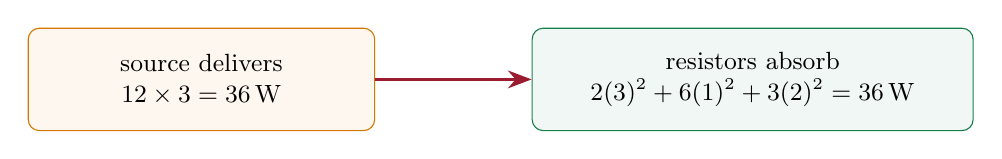
\begin{tikzpicture}[scale=1.0]
    \node[draw=cvolt, fill=cvolt!6, rounded corners=4pt, minimum width=4.4cm,
          minimum height=1.3cm, align=center, font=\small] (a) at (0,0)
         {source delivers\\ $12 \times 3 = 36\W$};
    \node[draw=cpow, fill=cpow!6, rounded corners=4pt, minimum width=5.6cm,
          minimum height=1.3cm, align=center, font=\small] (b) at (7.0,0)
         {resistors absorb\\ $2(3)^2 + 6(1)^2 + 3(2)^2 = 36\W$};
    \draw[flowarr] (a) -- (b);
  \end{tikzpicture}
  \end{center}
  \vfill
  \begin{center}\small\color{metugray}
    Costs one line and catches most sign errors.
  \end{center}
  \vfill
\end{frame}

%--------------------------------------------------------------
\begin{frame}{Summary}
  \vfill
  \begin{center}
  \begin{tabular}{@{}l l@{}}
    \toprule
    \textbf{KCL} \ $\sum \pm \Icol{i_k} = 0$ & at every node, every instant\\
    \textbf{KVL} \ $\sum \pm \Vcol{v_k} = 0$ & round every loop, every instant\\
    \bottomrule
  \end{tabular}
  \end{center}
  \vfill
  \begin{itemize}\itemsep5pt
    \item $2b$ unknowns $=$ $b$ \alert{terminal} $+$ $(n-1)$ KCL $+$ $(b-n+1)$ KVL.
    \item KCL holds on \alert{any closed surface}, not only at a node.
    \item KVL says \alert{voltage forgets the path}.
    \item Signs come from the \alert{reference} arrows and polarities you drew. You may
          pick them by guessing the true directions, but you need not --- a wrong guess
          costs nothing but a minus sign in the answer.
    \item Neither law knows what the elements are --- both survive nonlinear and
          time-varying circuits untouched.
  \end{itemize}
  \vfill
\end{frame}

%--------------------------------------------------------------
\begin{frame}{Next lecture}
  \vfill
  \begin{center}
  \begin{block}{What a two-terminal element can be}
    Independent voltage and current sources, the general definition of a resistor, and
    the five words for describing one --- all read off a curve in the $v$--$i$ plane.
  \end{block}
  \end{center}
  \vfill
  \begin{center}
    {\Large\color{metured} Questions?}\\[8pt]
    {\small Notes for this lecture: see the course repository.}
  \end{center}
  \vfill
\end{frame}

\end{document}
